\pgfplotsset{
  compat=1.16,
  % load a colormap that already included black
  % (either at the beginning or at the end)
  colormap/blackwhite,
  /pgf/declare function={
      u(\x,\y) = (1+0.5*y*cos(x/2))*cos(x);
      v(\x,\y) = (1+0.5*y*cos(x/2))*sin(x);
      w(\x,\y) = 0.5*y*sin(x/2);
  }
}

%
  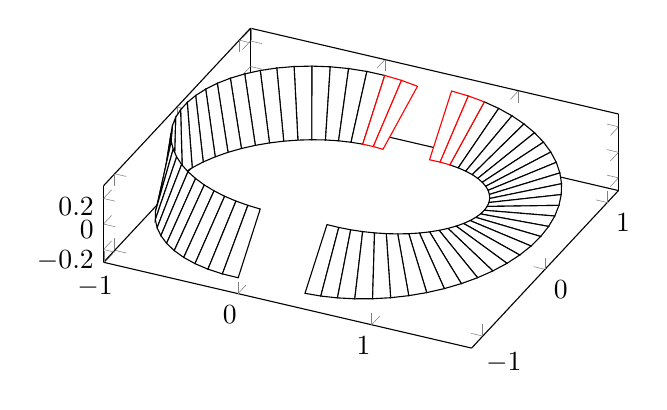
\begin{tikzpicture}
    \begin{axis}[
      %axis lines = none,
      axis equal image,
      trig format plots = rad,
      z buffer=sort
    ]
  \addplot3 [
      surf,
      shader=flat,
      draw=black,
      fill=white,
      point meta=x,
      samples=30,
      samples y=2,
      z buffer=sort,
      y domain=-0.5:0.5,
      fill=white,
      domain=pi/2:3*pi/2
  ] (
      {(1+0.5*y*cos(x/2))*cos(x)},
      {(1+0.5*y*cos(x/2))*sin(x)},
      {0.5*y*sin(x/2)});
  \addplot3 [
      surf,
      shader=flat,
      draw=red,
      fill=red,
      point meta=x,
      samples=3,
      samples y=2,
      z buffer=sort,
      y domain=-0.5:0.5,
      fill=white,
      domain=pi/2-0.21:pi/2
  ] (
      {(1+0.5*y*cos(x/2))*cos(x)},
      {(1+0.5*y*cos(x/2))*sin(x)},
      {0.5*y*sin(x/2)});
  \addplot3 [
      surf,
      shader=flat,
      draw=black,
      fill=white,
      point meta=x,
      samples=30,
      samples y=2,
      z buffer=sort,
      y domain=-0.5:0.5,
      fill=white,
      domain=3*pi/2:5*pi/2-0.21
  ] (
      {(1+0.5*y*cos(x/2))*cos(x)+0.5},
      {(1+0.5*y*cos(x/2))*sin(x)},
      {0.5*y*sin(x/2)});

  \addplot3 [
      surf,
      shader=flat,
      draw=red,
      fill=red,
      point meta=x,
      samples=3,
      samples y=2,
      z buffer=sort,
      y domain=-0.5:0.5,
      fill=white,
      domain=5*pi/2-0.21:5*pi/2
  ] (
      {(1+0.5*y*cos(x/2))*cos(x)+0.5},
      {(1+0.5*y*cos(x/2))*sin(x)},
      {0.5*y*sin(x/2)});
    \end{axis}

  \end{tikzpicture}